\title{Personalized Learning for practicing an English reading test}
\author{
  Donghee Hong \& Adrien Di Pasquale \\
  Department of Knowledge Service Engineering\\
  KAIST -- Daejeon, South Korea
}
\date{\today}

\documentclass[a4paper,12pt]{article}
\usepackage{hyperref}
\usepackage[utf8]{inputenc}
\usepackage{graphicx}
\usepackage{float}

\makeatletter
\def\maxwidth{%
  \ifdim\Gin@nat@width>\linewidth
    \linewidth
  \else
    \Gin@nat@width
  \fi
}
\makeatother

\begin{document}

\maketitle
\tableofcontents
\newpage


\section{Motivation}

Everyone has their own way of speaking, thinking, reacting. However, classic education systems are ``one size fits all'' : the same teacher, the same material and the same methodology for a given group of students. As freedoms and technologies evolve and allow knowledge to be less centralized, education is shifting towards new paradigms.

Personalized self-education (or autodidactism) is one solution to the ``one size fits all'' problem, as it allows a student to be independent and follow his own pace. The amount of resources available on the internet has also contributed to this method expansion. However, although you are free to choose the material you are going to use among those available, you usually cannot find or generate a truly customized material.

A key factor for successful education is motivation, and different students are not likely to be motivated by the same things. It is common to say that it is more motivating to learn something that relates to the real life, or to something interesting. It is indeed rewarding to be able to apply what you learn. However, all students have different life styles and activities, different interests.

Our general hypothesis is that students would be more motivated if the material relates to their daily life, their interests, or if the material is formatted in a way they appreciate.

Here are some examples of customized materials

\begin{enumerate}
\item a classic language lesson based on a dialog of a real life situations with the students' friends' names and pictures instead of fictional characters
\item a signal processing lesson providing examples for a song the student likes, or a photo, a video.
\item a lesson on a very abstract scientific matter mimicking the speech of someone the student likes, using a type of humour the student appreciates or a idiomatic sentences.
\end{enumerate}

These are three dissociated kinds of material customization : \textit{real-life}, \textit{interests} and \textit{taste}. These different methods could be more or less appropriate for different students, or different types of lessons. They could also have different impacts on the levels of student’s engagement and motivation and on the overall material efficiency (which is correlated).

Our research will try and assert that customized materials can be more efficient and engaging. We will not try to compare the different methods, but rather check that the common concept is valid.

Our research will focus on teaching English as a foreign language. This is a very appropriate field, since any of the customization methods can be easily applied. However, we will only explore customizing the material contents with the students' information and interests. Because of the complexity of such systems, we will not research customizing the materials' formats and style.


\section{Background - Related Work}

Though online learners can be diverse, from different backgrounds, and with a variety of different learning goals, motivations, learning skills and styles, most of the current web-based learning systems are still delivering the same educational resources in the same way to learners with different profiles [4]. Personalization involves using technology to accommodate these differences. It is becoming an increasingly important factor in education. However, it raises many technical and cognitive challenges. Many approaches have been attempted by researchers in the past decades.

Virtual Learning Environments (VLEs) are web-based systems that give a lot of freedom to the users and allow interaction. Researches have been conducted in this field to integrate personalization of the materials and learning plans. Xu and Wang developed a personalization model, implemented it in a VLE and tested its results \cite{xu_vle}. The outcome was that the personalized system yielded significantly higher scores for most of the tests, and that the students appreciated it more than the classical one.

Studies have been conducted to measure the personalization effects, especially on low level students. Cecilia and Howard investigated the effects of personalized instruction on the achievement of eighth-grade Mexican-American boys and girls from a rural junior high school on one-step and two-step mathematics problems \cite{lopez_hispanic}. The objective was to prove that personalizing story problems would make their context more familiar to the students, and therefore it improves their performance. The results of this research were significantly positive. It was also found that boys had lower results with standard materials than girls and that personalization increased their results more significantly than for girls. However, previous researchs had found that “Hispanic girls have commonly been found to have a more internal locus of control orientation than Hispanic boys”, which might reduce the scope of this result to this particular social environment.

Adaptive Learning is a field closely related to Personalized Instruction. It makes use of computers to deliver learning content that is personnaly adapted to the current learner. There are various sources of personalization information that can be used to create such content : the learning style, the cognitive style or learning achievement. A recent experiment run by Chung-Hua researchers (Taiwan) built an Adaptive Learning system and evaluated it \cite{tseng_two_sources}. Their approach was innovative : they mixed two sources of personalization information, whereas previous systems usually used a single one. The analysis of their results showed that both single-source and double-source systems could improve learning efficacy (as in whether learning is achieved or not). They also found out that only the double-source would significantly improve the learning efficiency (as in how much effort the students have to put in order to achieve learning).

There are also papers covering technical parts of the personalization process. Khribi \& Jemni investigated automatic personalization by profiling users on their web navigation history and preferences similarities \cite{khribi_recommendations}. They did not apply this personalization method to build an actual CBT System but instead computed personalized lists of recommended links to online materials. To do this they used information retrieval techniques and data mining on both the user profiles and the materials contents. It is however hard to evaluate their results, as it is often with IR systems.

In the field of teaching english as a foreign language, some approaches of personalized instructions were tested. Horie, Kashiwabara, Yamaguchi and Iijima developed a Glossary Generator \cite{iijima_wordlist_generator} that takes into account the students level and the materials difficulties. It also outputs some personalized teaching material where the words unknown to the current student are highlighted. It is effectiveness has not been measured, though. Closely related is Chen, Hsu, Li, and Peng's research paper : it models a learning system that recommends English news articles depending on the student's reading skills \cite{chen_mlearning}. They used a custom fuzzy algorithm to compute the student's skills based on their answers to short surveys.

These two last studies show interest for personalization in the field of foreign language teaching but they can only generate `simple' learning materials : lists of words or links. Generating a complete personalized material is a big challenge, as raised by Turker, Görgün and Conlan in ``The Challenge of Content Creation to facilitate Personalized eLearning Experiences'' \cite{turker_challenge_creation}. In this paper they introduce the European project iClass, a framework to build personalized eLearning systems. It provides services to model the user's profile and preferences and other services to generate personalized contents and learning strategies.


\section{Methods}

\subsection{Hypothesis}

\textit{``practicing with personalized learning materials compared to non-personalized learning materials will improve students scores on English reading comprehension test, because students will be more engaged with stories related to themselves''}

Vygotsky Learning theory includes the concept of a Zone of Proximal Development. In our experiment, we followed this concept : by transforming some of the complex context parts, we allow users to learn step by step. This approach should therefore yield better results than a traditional approach.

\subsection{Experiment}

Our test users will be around 30 KAIST students, only native Koreans. They are around 22 - 30 years old, have a strong scientific background and most of them also have a good level of english. We will aim at those with a TOEIC level under 890, because it has been noted that lower level students tend to be more sensitive to personalization.

Our experiment is composed of 5 steps : \textit{registration}, \textit{pre-test}, \textit{practice}, \textit{post-test}, and \textit{questionnaire}. The pre-test will be performed unmonitored at home, about one week before the experiment. The training and post-test will take place in the lab, under our supervision. For the training step, the students will be divided in two groups : the control group will use standard materials and the study group will use personalized ones (between group test). During this central step, we will measure the time spent, the results and the students' attitudes. None of the 5 steps will have a time limit, however for the pre and post-tests only, we will tell the students that they should complete it quickly, as in a real test. For the pre and post-tests we will use standard materials for both groups. The reason for this is that we want our experiment to focus on the results of personalized vs standard training materials for a real-life test (hence a standard test).

The customized material will be generated for each student based on personal information like the name, age, address, but also on personal interests or point of views : more of a family person or career oriented, would like to live close to the beach or the mountain, have a strong passion for music … Students will fill an online form to let us know this. Only the Study Group data is going to be used, but for equity the other group will take this survey as well. Our standard materials will consist of TOEIC step 7 tasks, slightly incremented with context sentences. These sentences will be as neutral as possible : they should not help the students answer the questions. Then, the personalized materials will be generated by replacing these new context sentences contents (and other pre-existing identified context sentences) with contents based on the user profile.

The task consists of a document of about 100 words, often a letter, but sometimes an ad or another piece of informative paper, and several questions related to it. The questions all have multiple choices answers. They are usually not straightforward questions, so you have to understand the whole context, and also some implicit meanings. This task is copied on TOEIC's part 7.

However the whole process, pre and post-tests training, and tests will be performed on a web-based interface, which removes the classic paper interaction (underlining, circling ..) and might make the task more difficult. We still believe it is better to do it this way, since most of the personalized systems available today are web-based, and also because being able to read fluently on a screen is a useful skill.


\section{Results (of the pilot test)}

We did not have the time or the resources to conduct the whole experiment as planned. However, we did perform a pilot test with 4 test users matching our criterias. This provided us with valuable feedbacks for the interface, and let us confirm or reject our experimental design.

We wrote a R script to analyze statistically the results of the experiment.
The results we show below come from running this script on our pilot test data, and should therefore \textit{NOT} be interpreted as statistically strong, considering the very low number of test users.

Here is an informative graph of the mean ratio of correct answers for the control (traditional material) and test (personalized material) groups :

\begin{figure}[H]
\begin{center}
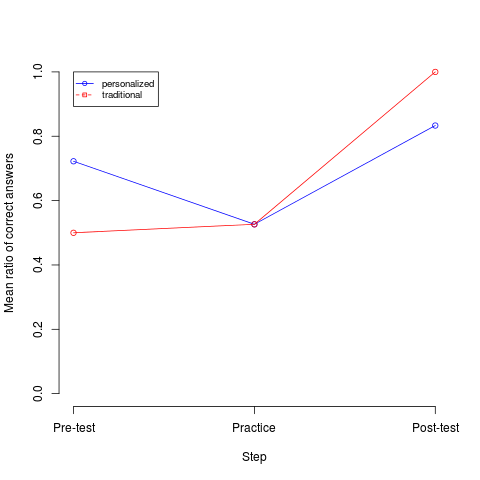
\includegraphics[width=10cm]{means.png}
\caption{Mean ratio of correct answers}
\label{means}
\end{center}
\end{figure}

We can see that the personalized material has globally yielded better results.

We then performed a Welch T-Test that tests the null hypothesis that the means of the control and test groups have the same mean. The resulting p-value is 0.33, which doesn't allow us to conclude that the means are different.


\section{Extra Material : Prototype Presentation}

\subsection{Why build a website ?}

Creating the personalized material for each of our students would be very time consuming without the help of a computer. Moreover, we have to make sure that the Personalized and Traditional materials vary only on very specific parts and in specific ways. Doing it manually could result in a natural tendency to cross these boundaries, and personalize bigger parts of the material. Using an algorithm allows us to be 100\% sure of the extent of the personalization.

Our task (TOEIC exercise type 7) is very well suited for a computer use : it does not require any interaction with an instructor, and the submission of a simple form of checkboxes fully characterizes an answer.

It is actually common to perform these tasks on a computer : TOEIC computer-based training softwares are widely available. It is also very probable that the test itself will soon be performed using computers.

A paper-based version of this task would have had a single extra benefit : the ability to highlight and annotate the material, which students often find useful.

\subsection{Website walkthrough}

\subsubsection{At Home}

The first step can be done by the user at his/her home. This allows to reduce the in-lab steps complexity and duration.

\begin{enumerate}

\item The user receives a mail

This mail is an invitation to join the experiment. It contains a link to the website and a predefined login. Users should follow the link and sign in using this login. They will then see a welcome message and a single link towards the profile form.

Some general remarks about the website at this point : it has a minimalist design, and a lot of space. Font sizes are used to emphasize on the important
parts. The header color depends on the user's current step.

\item The user fills his / her profile

It is composed of various fields on different personal information : age, size, hobby, favourite artist … The fields are either open or provide a fixed set of choices.

All the users have to go through this step, even those who will be put in the control group. This ensures equity over the two groups : the students should not directly know which group they belong to.

After filling this form, the website displays a message reminding them of the rendez-vous time and location for the following in-lab steps.
\end{enumerate}

\begin{figure}
\begin{center}
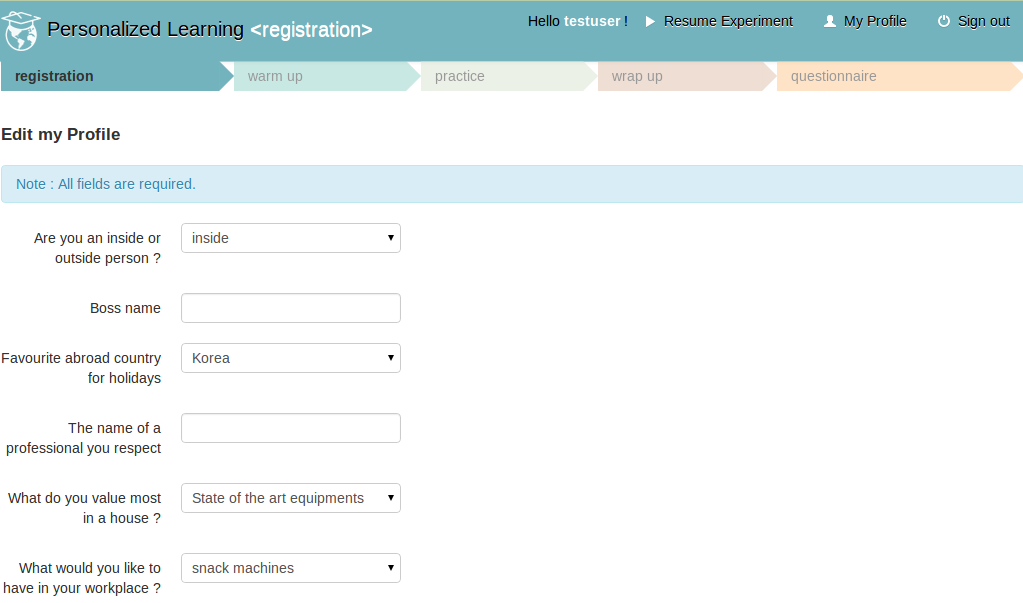
\includegraphics[width=\maxwidth]{registration.png}
\caption{User profile page}
\label{means}
\end{center}
\end{figure}


\subsubsection{In the Lab}

The biggest part of the experiment will then be run in the lab. Students will be welcomed in groups of 4 to perform the task. We will first introduce them to the process, and then let them go through it on their own.

\begin{enumerate}

\item Pre-test

First students will have to log in again to the website, so that they can fetch back the profile data they input previously. Then, they will have to perform a post-test task, cf. Figure \ref{pre_test}. This task will provide Traditional material for both groups. We will record the time, but will not set a limit.

We used less than 4 colours for the interface in order to not distract the user from the material. We have not put any colours in the materials, to mimic the real-life tests.

\begin{figure}
\begin{center}
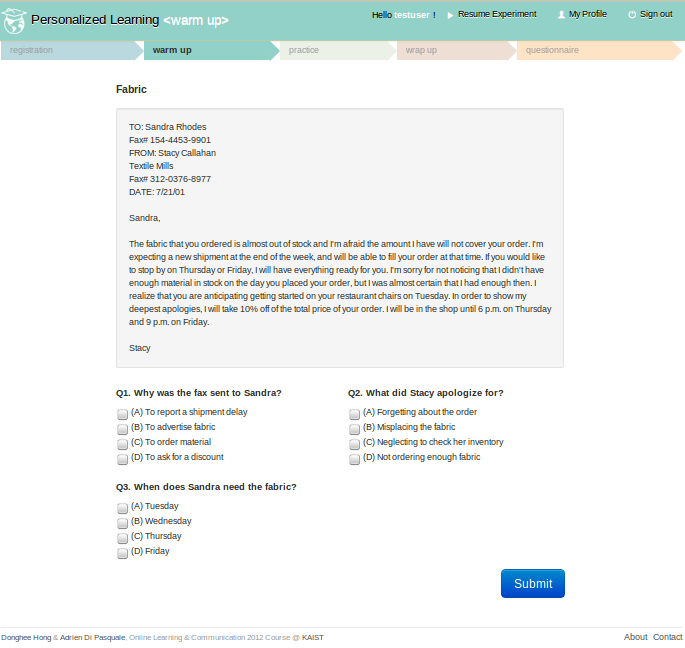
\includegraphics[width=\maxwidth]{pre_task.png}
\caption{Pre test task}
\label{pre_test}
\end{center}
\end{figure}

\item Practice

Students will then be presented with 10 Practice tasks, that will have Traditional material for the Control group and Personalized material for the other. There will be no timing of this step, but they will have to complete in a certain amount of time. We will allow them to take breaks but no to have discussion among them, as to not bias the experiment.

\item Post-test

This step is almost exactly the same as the Pre-test : Traditional material, time measured but not limited.

\item Questionnaire

After the post test, we will ask students to take the questionnaire we wrote. Its purpose is mainly to evaluate how familiar they felt during practice, and measure their perceived engagement.
It also includes two open feedback questions, that they can optionally fill.

\end{enumerate}


\subsubsection{Backend}

The website is a complete platform, as it provides a complete backend to edit Tasks (cf. figure \ref{edit_task}) and Questionnaires, and to handle Users (creation, step \& material type assignment ..).

The forms can get a bit complicated because a big flexibility is required to input the Personalizable parts possible values, in the Tasks material, Questions texts and choices … We will not get into details in this document but the website provides some on-screen indications, and more information can be found using the resources listed in the next section


\begin{figure}
\begin{center}
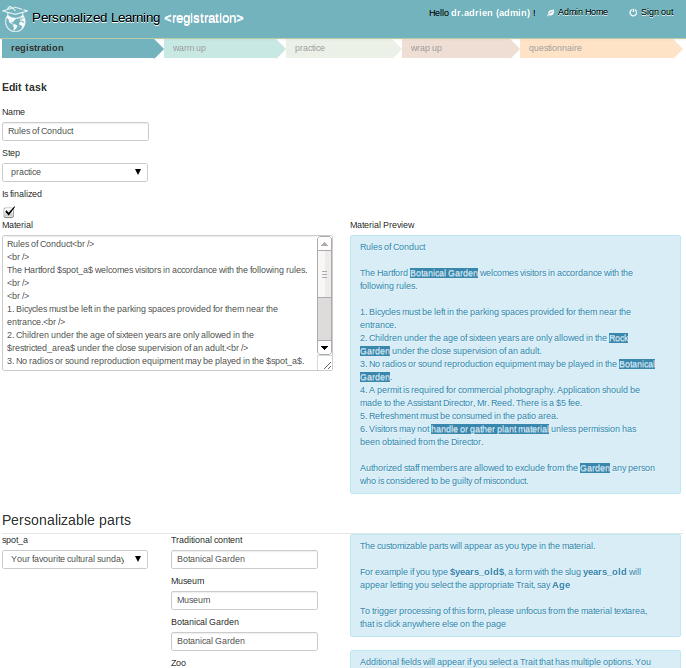
\includegraphics[width=\maxwidth]{edit_task.png}
\caption{Backend - Edit task}
\label{edit_task}
\end{center}
\end{figure}


\subsection{External reference}

The prototype source code and an online demo version can be found there :
\url{http://github.com/adipasquale/personalized_learning}

It can freely be forked for any similar experiment.

\bibliographystyle{abbrv}
\nocite{*}
\bibliography{experiment_report}

\end{document}